El experimento Solenoide Compacto de Muones o \CMS(\textbf{C}ompact \textbf{M}uon \textbf{S}olenoid) tiene la capacidad de cubrir un amplio rango de procesos físicos, este experimento consiste de varios subsistemas los cuales están diseñados para la identificación de prácticamente todas las partículas del modelo estándar. Para su diseño se tomó en cuenta cómo cada partícula interacciona con la materia, por ejemplo las partículas cargadas son identificadas por medio de detectores a base de silicio y de gas noble, permitiendo determinar con precisión el tiempo y localización de las partículas. La variedad de interacciones por tipo de partícula se puede ver en la Fig. \ref{cms}.

\begin{figure}
\centering
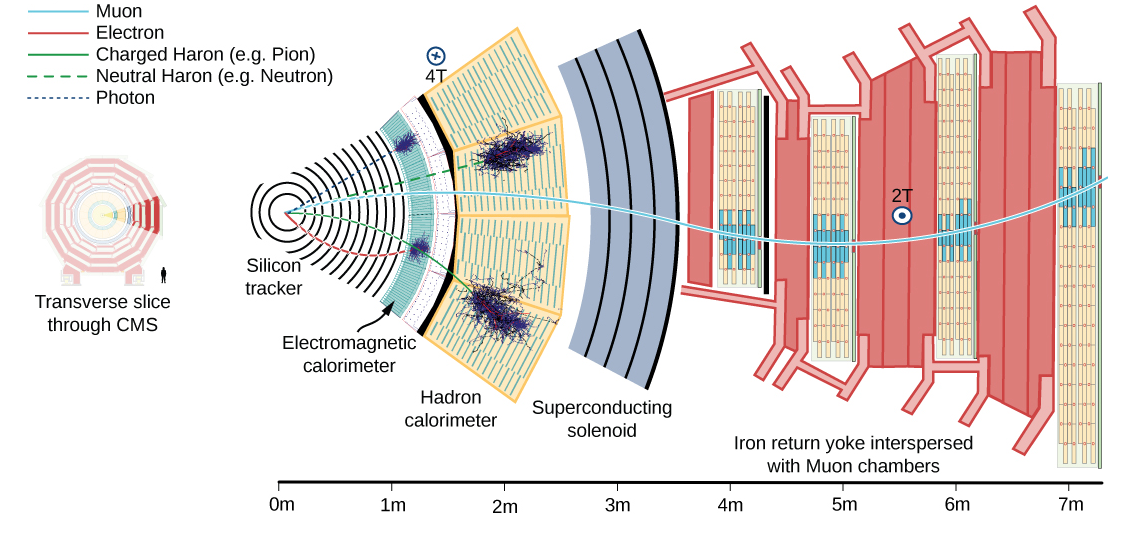
\includegraphics[width=1\textwidth]{Analisis_y_Resultados/imagenes/CMS_interaction.png}
\caption{Detector de solenoide de muón compacto. El detector consta de varias capas, cada una responsable de medir diferentes tipos de partículas. Pagina de origen: \url{http://ippog.web.cern.ch/resources/2011/cms-slice-july-2010-version}.}
\label{cms}
\end{figure}

El CMS es un detector de propósito general, capaz de estudiar múltiples aspectos de las colisiones de protones hasta 14 TeV. También contiene sistemas para medir la energía y la cantidad de movimiento de fotones, electrones, muones y otras partículas producto de las colisiones. La capa detectoras se pueden dividir en: 
\begin{itemize}
\item[-]  \textbf{El rastreador de Silicio (The Silicon tracker) :} para calcular el momento de una partícula es rastrear su camino a través de un campo magnético; cuanto más curvaba el camino, menos impulso tenía la partícula. El rastreador \CMS registra los caminos tomados por las partículas cargadas al encontrar sus posiciones en varios puntos clave. De esta forma se reconstruyen los caminos de muones de alta energía, electrones y hadrones (partículas formadas por quarks), así como ver las huellas que provienen de la descomposición de partículas de vida muy corta.

El rastreador \CMS ~ está hecho completamente de silicio: los píxeles, en el núcleo mismo del detector y que se ocupan de la mayor intensidad de partículas, y los detectores de microstrip de silicio que lo rodean. A medida que las partículas viajan a través del rastreador, los píxeles y las microstrips producen pequeñas señales eléctricas que se amplifican y detectan. El rastreador emplea sensores que cubren un área del tamaño de una cancha de tenis, con 75 millones de canales de lectura electrónica separados: en el detector de píxeles hay unas 6,000 conexiones por centímetro cuadrado.

\textbf{Actualización de Alta Luminosidad : }

La actualización esperada de \textbf{HL-}\LHC~ aumentará el número de interacciones hasta el punto en que la ocupación excesiva reduciría significativamente la efectividad de la búsqueda de pistas. Se planea una actualización para aumentar el rendimiento y la tolerancia a la radiación del rastreador.

\item[-] \textbf{Calorímetro electromagnético} o \textbf{ECAL} (\textbf{E}lectromagnetic \textbf{CAL}orimeter) : componente diseñado para medir con alta precisión las energías de electrones y fotones, está construido a partir de cristales de plomo tungstato ($PbWO_4$). Este es un material extremadamente denso pero ópticamente transparente, ideal para detener partículas de alta energía, este material está hecho principalmente de metal y es más pesado que el acero inoxidable, pero con un toque de oxígeno en esta forma cristalina es muy transparente y centellea cuando los electrones y fotones lo atraviesan, lo que produce luz en proporción a la energía de la partícula. Para mayor precisión espacial, el \textbf{ECAL} también contiene detectores de ``preshower'' que se encuentran frente a las tapas finales, permitiendo distinguir entre fotones individuales de alta energía (a menudo signos de física emocionante) y los pares cercanos menos interesantes de fotones de baja energía. Está calibrado para discriminar entre de piones y fotones.

\item[-] \textbf{El calorímetro de hadrones} o \textbf{HCAL}(\textbf{H}adronic \textbf{CAL}orimeter) : mide la energía de los hadrones, además, proporciona una medición indirecta de la presencia de partículas no cargadas que no interactúan, como los neutrinos. Consta de capas de material denso (latón o acero) intercaladas con baldosas de centelleadores de plástico, leídas a través de fibras que cambian la longitud de onda mediante fotodiodos híbridos, de esta forma se permite la máxima cantidad de material absorbente dentro de la bobina magnética.

\item[-] \textbf{Solenoide supercondutor (Superconducting Solenoid):} es el dispositivo central alrededor del cual se construye el experimento, con un campo magnético de 4 Tesla permite determinar la relación carga/masa de partículas a partir de la pista curva que siguen en el campo magnético. Tiene $13~m$ de largo y $6~m$ de diámetro, y sus bobinas de niobio-titanio superconductoras refrigeradas estaban destinadas originalmente a producir un campo magnético de hasta $4~T$. Es componente tiene la función de doblar los caminos de las partículas que emergen de colisiones, permitiendo determinar con la trayectoria curvada por el campo magnético el impulso, combinado con mediciones de posición de alta precisión en los rastreadores y detectores de muones, esto permite una alta medición en sus resultados.

\item[-] \textbf{Los detectores de muones :} dedicado a la detección de muones, siendo estas partículas cargadas y 200 veces más masivas que los electrones y positrones, se espera que se produzcan en la descomposición de una serie de posibles partículas nuevas. Debido a que los muones pueden penetrar varios metros de hierro sin interactuar, ninguno de los calorímetros de \CMS ~los detiene. Por lo tanto, las cámaras para detectar muones se colocan en el borde mismo del experimento, donde son las únicas partículas que pueden registrar una señal. Para identificar muones y medir sus momentos, \CMS ~ utiliza tres tipos de detectores: 
\begin{itemize}
\item \textbf{Tubos de deriva} o \textbf{DT}(\textbf{D}rift \textbf{T}ubes) : se usan para mediciones de trayectoria precisas en la región central del barril.
\item \textbf{Cámaras de banda catódica} o \textbf{CSC}(\textbf{C}athode \textbf{S}trip \textbf{C}hambers) : se usan para mediciones de trayectoria precisas en los extremos del barril. 
\item \textbf{Cámaras de placas resistivas} o \textbf{RPC}(\textbf{R}esistive \textbf{P}late \textbf{C}hambers) : proporcionan una señal rápida cuando un muón pasa a través del detector.
\end{itemize}

\end{itemize}
